\documentclass[12pt,letterpaper,titlepage]{report}
\usepackage[latin1]{inputenc}
\usepackage{amsmath}
\usepackage{amsfonts}
\usepackage{amssymb}
\usepackage{graphicx}
\usepackage{pdfpages}
\usepackage{float}
\usepackage{titlesec}
\usepackage{needspace}
\usepackage{hyperref}
\usepackage[width=8.50in, height=11.00in, left=1.00in, right=1.00in, top=1.00in, bottom=1.00in]{geometry}
\usepackage[backend=bibtex,style=ieee]{biblatex}

% Default fixed font does not support bold face
\DeclareFixedFont{\ttb}{T1}{txtt}{bx}{n}{12} % for bold
\DeclareFixedFont{\ttm}{T1}{txtt}{m}{n}{12}  % for normal

% Custom colors
\usepackage{color}
\definecolor{deepblue}{rgb}{0,0,0.5}
\definecolor{deepred}{rgb}{0.6,0,0}
\definecolor{deepgreen}{rgb}{0,0.5,0}

\usepackage{listings}

% Python style for highlighting
\newcommand\pythonstyle{\lstset{
		language=Python,
		basicstyle=\ttm,
		otherkeywords={self},             % Add keywords here
		keywordstyle=\ttb\color{deepblue},
		emph={MyClass,__init__},          % Custom highlighting
		emphstyle=\ttb\color{deepred},    % Custom highlighting style
		stringstyle=\color{deepgreen},
		frame=tb,                         % Any extra options here
		showstringspaces=false            % 
}}

% Python environment
\lstnewenvironment{python}[1][]
{
	\pythonstyle
	\lstset{#1}
}
{}

% Python for external files
\newcommand\pythonexternal[2][]{{
		\pythonstyle
		\lstinputlisting[#1]{#2}}}

% Python for inline
\newcommand\pythoninline[1]{{\pythonstyle\lstinline!#1!}}

% Variables
\titleformat{\section}
{\needspace{8\baselineskip}\Large\bfseries}{\thesection}{1em}{}


% Document start ~~~~~~~~~~~~~~~~~~~~~~~~~~~~~~~~~~~~~~~~~~~~~~~~~~~~~~~~~~~~~~~~~~~~~~~~~~~~~~~~~~~~~

\title{Neural network-based controller}
\author{Justin Ng}
\bibliography{bib} 

\begin{document}
\pagenumbering{gobble}
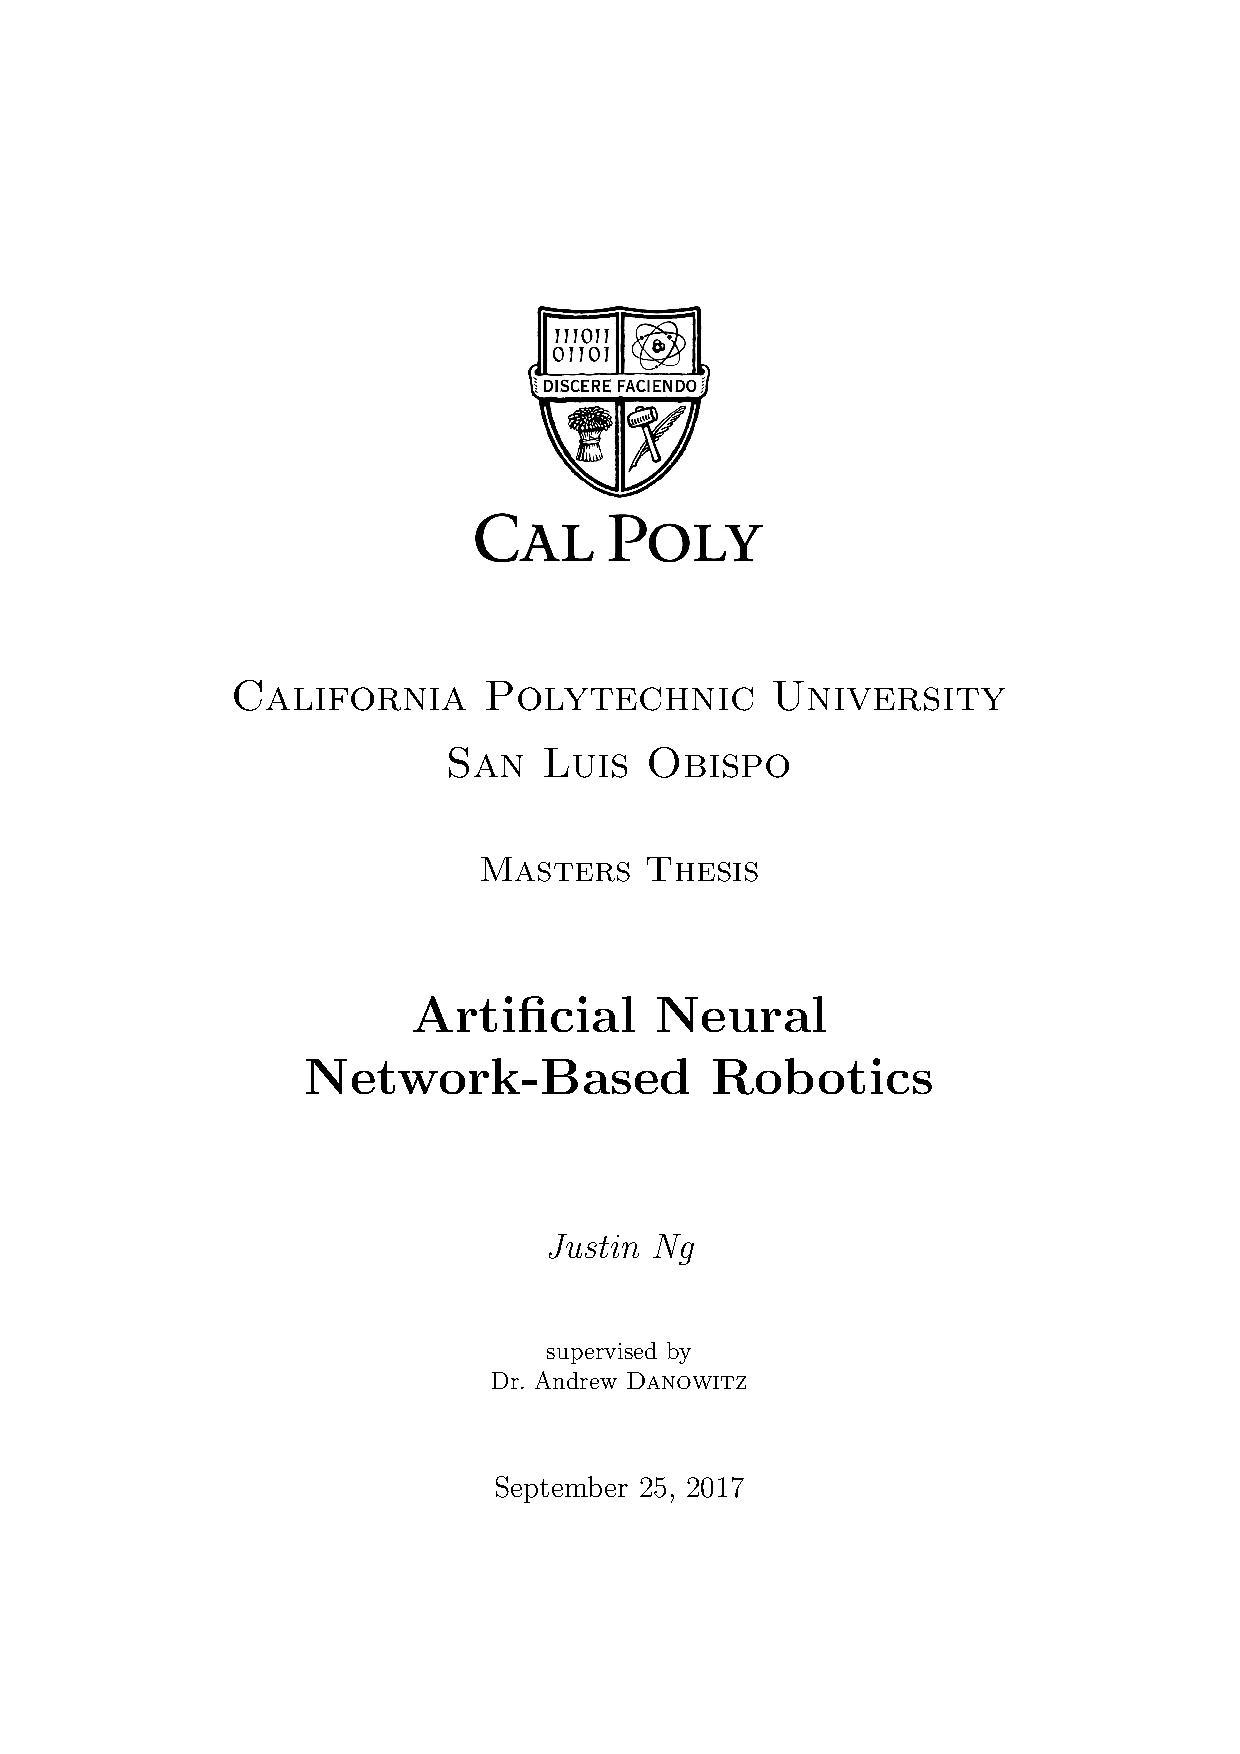
\includepdf{titlepage}
\newpage
\pagenumbering{roman}
\tableofcontents
\listoffigures
\listoftables


\chapter*{Acknowledgements}
\addcontentsline{toc}{chapter}{Acknowledgements}
I would like to thank everyone for everything.


\chapter*{Abstract}
\addcontentsline{toc}{chapter}{Abstract}
\textbf{Note}: All project files can be found at \url{https://www.github.com/okayjustin/roborodentia2017} \

Artificial neural networks (ANNs) are highly-capable alternatives to traditional problem solving schemes due to their ability to solve non-linear systems with a non-algorithmic approach. The applications of ANNs range from process control to pattern recognition and, with increasing importance, robotics. A robot is created with multiple sensors and actuators for environment perception, movement and object manipulation while an on-board microcontroller processes the ANNs and provides the control interface. After training, the neural networks use the various sensor inputs to make the robot accomplish a series of tasks. The system demonstrates how effective and applicable ANNs are to robotic control. 


\chapter{Introduction}
\section{Kalman Filters}
The system relies on several different sensors to determine where it is within the environment, a problem commonly referred to as robot localization. The \textit{Kalman Filter} (KF), an optimal state estimator, performs noise filtering and sensor fusion, the process of combining measurements from multiple sensors. 

\subsection{Algorithm}
The Kalman Filter algorithm and equations are reproduced here from Roger Labbe's excellent interactive, online book \autocite{labbe_2017}.
\subsubsection*{Initialization}
Before the first run of the filter, initialize the estimated state (\textbf{x}, also called the prior) and estimated state covariance matrix (\textbf{P}).
\subsubsection*{Predict}
During the predict phase, the process model is used to predict the future state (\textbf{\=x}, prior) after one time step by summing the current estimated state (\textbf{x}) multiplied by the \textit{state transition function} (\textbf{F}) with the xxxxxxx (\textbf{B}) multiplied by the xxxxxx(\textbf{u}). The covariance of prior (\textbf{\=P}) is larger than the estimated state covariance (\textbf{P}) due to uncertainty in the process model (\textbf{Q}).
\begin{align*}
\bar{\textbf{x}} &= \textbf{Fx} + \textbf{Bu}\\
\bar{\textbf{P}} &= \textbf{FPF}^T + \textbf{Q}\\
\end{align*}

\subsubsection*{Update}
Make measurements (\textbf{z}, measurement mean) and determine their accuracy (\textbf{R}, measurement noise covariance). Calculate the residual (\textbf{y}) between the measurement and the product of the measurement function (\textbf{H}) and the predicted state from the previous phase. Calculate the scaling factor (\textbf{K}, Kalman gain) based on whether the measurement or predicted state is more accurate. Set the next estimated state, \textbf{x}, between the measurement and predicted state based on \textbf{K}. Finally, update the estimated state covariance, \textbf{P}, based on the certainty in the measurement.
\begin{align*}
\textbf{y} &= \textbf{z} - \textbf{H}\bar{\textbf{x}}\\
\textbf{K} &= \bar{\textbf{P}}\textbf{H}^T(\textbf{H}\bar{\textbf{P}}\textbf{H}^T+\textbf{R})^{-1}\\
\textbf{x} &= \bar{\textbf{x}} + \textbf{Ky}\\
\textbf{P} &= (\textbf{I}-\textbf{KH})\bar{\textbf{P}}\\
\end{align*}

\pagenumbering{arabic}
\chapter{Project Plan (draft)}
\section{Problem}
Create a competition robot for Roborodentia and control it using neural networks.

\section{Solution}
Design and manufacture a robot. Write firmware with a neural network implementation and train it to perform competition tasks. 

\section{Objectives}
\begin{itemize}
	\item Select robot design criteria.
	\item Create several solutions and prototype a few proof-of-concepts.
	\item Design electrical systems:
	\begin{itemize}
		\item Power systems: Batteries, regulation, distribution.
		\item Microcontroller: sufficient processing power and IO.
		\item Sensors: dependent on control strategy. What information needed?
		\item Actuators
	\end{itemize}
	\item Model robot in SolidWorks with attention to manufacturing.
	\item Order parts and manufacture robot.
	\item Bring up electrical system and perform functional checks.
	\item Design neural network and training plan.
	\item Develop firmware: neural network, FSM design, communications, debug code.
	\item Train network and tune.
	\item Revise mechanical/electrical/firmware and repeat.
\end{itemize}


\section{Tasks and Timeline}



\chapter{\LaTeX\ Usage}

\section{Figures and Ref}
This is where I introduce stuff. See Figure \ref{fig:padthai}.

\begin{figure}[H]   % [h] means here
	\centering
	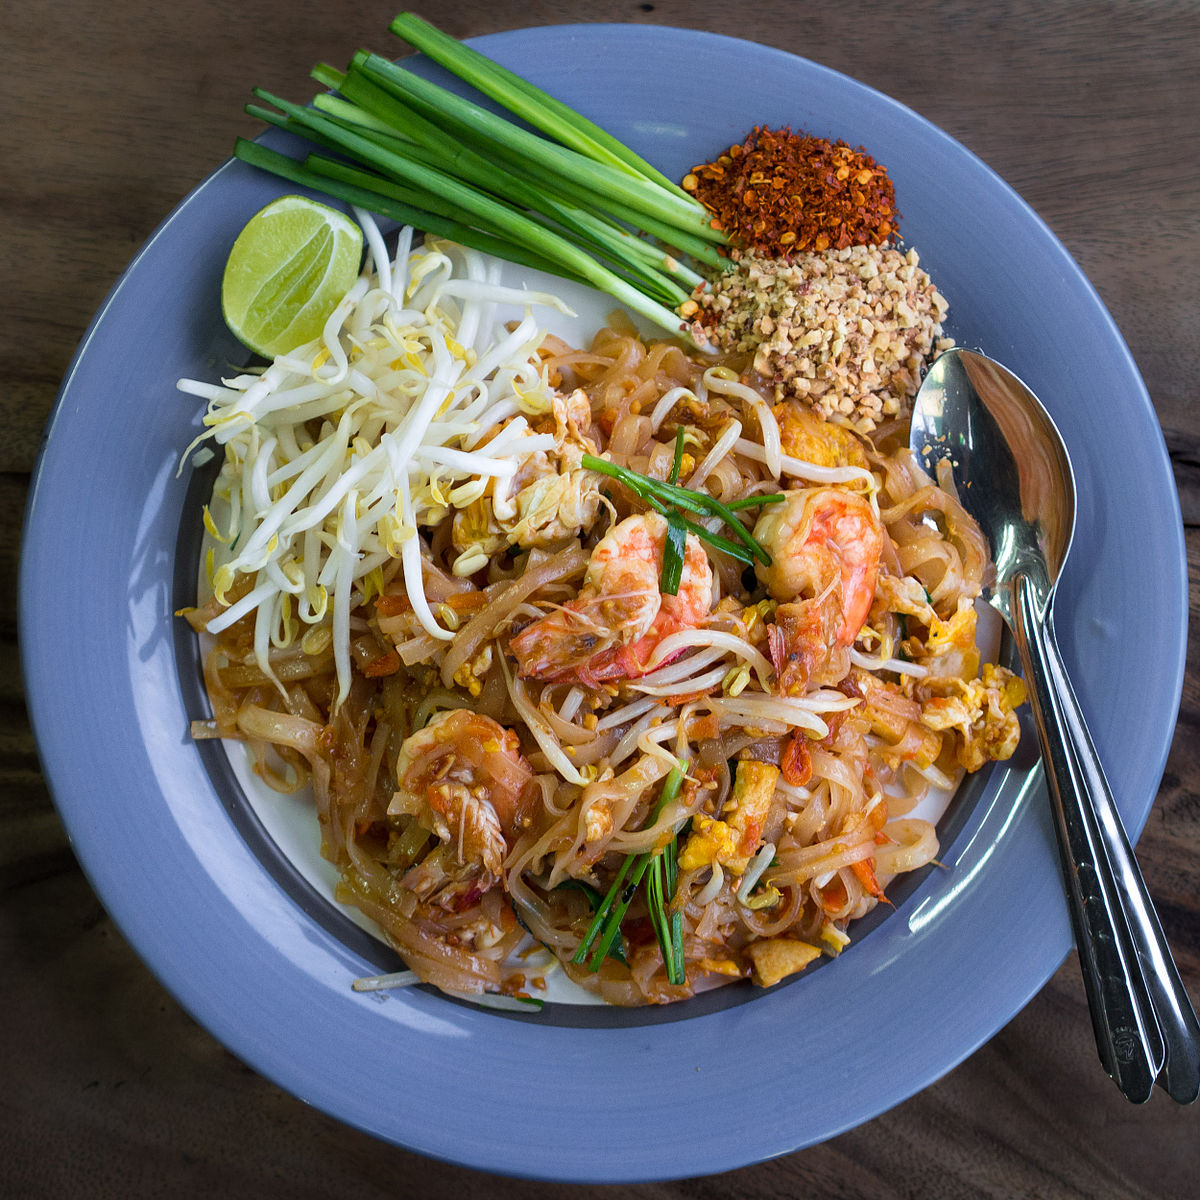
\includegraphics[width=3.6in]{images/padthai.jpg}
	\caption{Pad thai}
	\label{fig:padthai}
\end{figure}



\section{Math}

\begin{equation}
	f(x) = x^2
\end{equation}


This is an equation that we don't want to number: $$f(x) = x^2$$

Here's an in-line equation: $f(x) = x^2$.

Here's an aligned equation: Aligns at the \&.
\begin{align*}
	1 + 2 & = 3                       \\
	1     & = 3 - 2                   \\
	f(x)  & = x^2                     \\
	g(x)  & = \frac{1}{x}             \\
	F(x)  & = \int^a_b \frac{1}{3}x^3 \\
	\frac{1}{\sqrt{x}}
\end{align*}

\[\begin{bmatrix}
		a & \lambda \\
		c & d
	\end{bmatrix}\]



\section{Citations}


Random citation \autocite{nguyen_widrow_1990} embeddeed in text.

Random citation \autocite{DUMMY:1} embeddeed in text.

Random citation \autocite{nguyen_widrow_1990} embeddeed in text.
\autocite{negenborn_2003} \autocite{labbe_2017}

\section{Accents}

Premi\`ere	\.x

\section{Dashes}

The space is 3-dimensional.

Read pages 3--4.

I saw them---there were 3 men alive

The temperature dropped to $-$3 degrees.

\section{Lists}

\begin{itemize}
	\item  First Level
	      \begin{itemize}
		      \item  Second Level
		            \begin{itemize}
			            \item  Third Level
			                  \begin{itemize}
				                  \item  Fourth Level
			                  \end{itemize}
		            \end{itemize}
	      \end{itemize}
\end{itemize}
\begin{enumerate}
	\item First level item
	\item First level item
	      \begin{enumerate}
		      \item Second level item
		      \item Second level item
		            \begin{enumerate}
			            \item Third level item
			            \item Third level item
			                  \begin{enumerate}
				                  \item Fourth level item
				                  \item Fourth level item
			                  \end{enumerate}
		            \end{enumerate}
	      \end{enumerate}
\end{enumerate}

\section{Groups}
 {
  \hsize = 4 in
  \parindent = 0 pt
  \leftskip = 1 in
  will produce a paragraph that is four
  (this is an easy mistake to make).
  \par
 }


\section{Code highlighting}

\begin{python}
	class MyClass(Yourclass):
	def __init__(self, my, yours):
	bla = '5 1 2 3 4'
	print bla
\end{python}


\chapter{Control Problem}

\chapter{Training Algorithm}

\chapter{Implementation}

\chapter{Results}

\chapter{Conclusion}

\renewcommand\bibname{References}
\printbibliography
\addcontentsline{toc}{chapter}{References}

\chapter*{Appendices}
\addcontentsline{toc}{chapter}{Appendices}


\end{document}